%%%%%%%%%%%%%%%%%%%%%%%%%%%%%%%%%%%%%%%%%%%%%%%%%%%%%%%%%%%%%%%%%%%%%%%%%%%%%%%%
% > Лабораторная работа 6: Критические угловые скорости гибкого вала.
% > Баталов Семен, Антонова Мария, Клюшин Максим, Хайретдинова Диана.
% > 2021 год.
%%%%%%%%%%%%%%%%%%%%%%%%%%%%%%%%%%%%%%%%%%%%%%%%%%%%%%%%%%%%%%%%%%%%%%%%%%%%%%%%

\documentclass[12pt, a4paper]{article}
\usepackage[left=2cm, right=2cm, top=2.5cm, bottom=2.5cm, nohead, 
footskip=1cm]{geometry}
\usepackage{graphicx}
\graphicspath{{./Pictures/}}
\usepackage[utf8]{inputenc}
\usepackage[english, russian]{babel}
\usepackage{indentfirst}
\usepackage{array}
\usepackage{longtable}
\usepackage{misccorr}
\usepackage{setspace, amsmath}
\usepackage{multirow}

\begin{document}
    
    \newcolumntype{M}[1]{>{\centering\arraybackslash}m{#1}}
    \renewcommand{\arraystretch}{1.4}
    
    \begin{center}
        \large{Санкт-Петербургский государственный университет} \\
        \large{Saint-Petersburg State University}\\
        \hfill \break
        \hfill \break
        \hfill \break
        \hfill \break
        \hfill \break
        \hfill \break
        \hfill \break
        \large{Кафедра теоретической и прикладной механики} \\
        \hfill \break
        \hfill \break
        \large{\textbf{ОТЧЕТ}} \\
        \large{\textbf{По лабораторной работе 6}} \\
        \large{<<Критические угловые скорости гибкого вала>>} \\
        \hfill \break
        \hfill \break
        \hfill \break
        \large{По дисциплине} \\
        \large{<<Лабораторный практикум по теоретической механике>>} \\
    \end{center}
    
    \hfill \break
    \hfill \break
    \hfill \break
    \hfill \break
    \hfill \break
    \hfill \break
    
    \begin{flushright} 
        \large{Выполнили:} \\
        \hfill \break
        \large{Баталов С. А.} \\
        \large{Антонова М. Н.} \\
        \large{Клюшин М. А.} \\
        \large{Хайретдинова Д. Д.} \\
    \end{flushright}
    
    \hfill \break
    \hfill \break
    \hfill \break
    \hfill \break
    
    \begin{center} 
        \large{Санкт-Петербург} \\
        \large{2021} \\
    \end{center}
    
    \thispagestyle{empty}
    \newpage
    \sloppy
    
    \section{Описание установки}
    
    В данной работе рассматривается явление потери устойчивости прямолинейной формы вращающегося вала. Целью работы является экспериментальное определение первых двух критических угловых скоростей, наблюдение соответствующих форм потери устойчивости и сравнение полученных результатов с теоретическими.
    
    \begin{figure} [h]
        \centering
        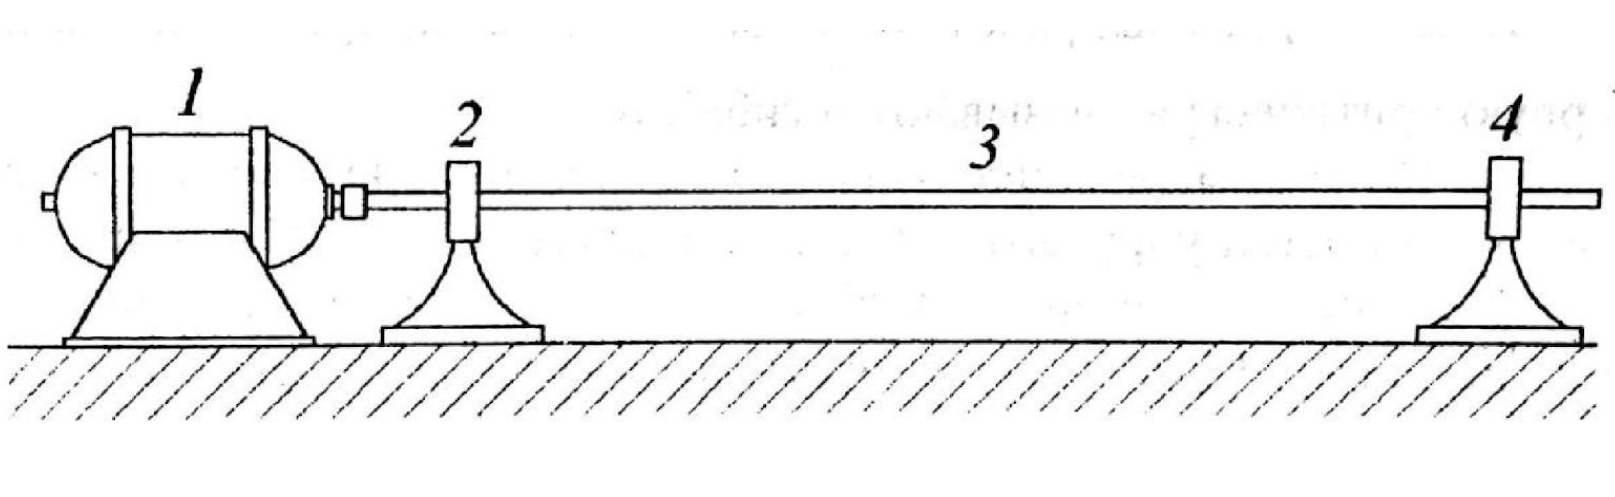
\includegraphics [width = 13cm] {Lab_6_1.png}
        \caption{\centering Схема лабораторной установки.}
        \label{im1}
    \end{figure}
    
    На рис.~\ref{im1} изображена схема лабораторной установки. Основной частью установки является гибкий деревянный вал \textit{3}, установленный на станине в двух сферических подшипниках \textit{2} и \textit{4}. Вал может скользить вдоль оси подшипника \textit{4}. Описанный способ крепления дает валу возможность вращаться не только в прямолинейном, но и в изогнутом состоянии. Вал \textit{3} связан с валом электродвигателя \textit{1}, находящегося на станине.
    
    \newpage
    
    \section{Параметры установки}
    
    В следующей таблице представлены параметры установки и замерочного вала: длина образца~--~$l^{*}$, масса образца~--~$m^{*}$, модуль упругости материала вала~--~$E$, диаметр вала~--~$d$, длина вала~--~$l$.
    
    \begin{longtable}{ | M{2cm} | M{3cm} | M{3cm} | M{3cm} | M{3cm} |}
        \caption{\centering Результаты измерений параметров установки.}
        \label{tb1} \\
        \hline
        Номер & Величина & Значение & Погрешность & Размерность \\
        \hline
        1 & $d$ & 0,018 & 0,0005 & м \\
        2 & $l$ & 1,970 & 0,001 & м \\
        \hline
        3 & $l^{*}$ & 0,126 & 0,0005 & м \\
        4 & $m^{*}$ & 0,022 & 0,0005 & кг \\
        \hline
        % 3 & $\rho$ & 667 & -- & $\text{кг} / \text{м}^{3}$ \\
        5 & $E$ & $1,38 \cdot 10^{10}$ & -- & Па \\
        \hline
    \end{longtable}
    
    \newpage
    
    \section{Теоретические исследования}
    
    В данном разделе приведем теоретическое описание процесса вращения упругого вала с различными угловыми скоростями. Для начала требуется найти линейную плотность материала вала~--~$p$. Для этого воспользуемся формулой (\ref{eq1}).
    
    \begin{equation}
        p = \frac{m}{l} = \frac{m^{*}}{l^{*}}.
        \label{eq1}
    \end{equation}
    
    Так же нужно расчитать момент инерции $I$ площади поперечного сечения вала относительно его диаметра по формуле (\ref{eq2}).
    
    \begin{equation}
        I = \frac{\pi r^{4}}{4} = \frac{\pi d^{4}}{64}.
        \label{eq2}
    \end{equation}
    
    Для нахождения критической угловой скорости составим дифференциальное уравнение изогнутой осри вала для однородной балки постоянного сечения. Запишем это уравнение (\ref{eq3}) и продифференцируем два раза по $x$, где $x$~--~ось стержня. После этого упростим до вида (\ref{eq4}).
    
    \begin{equation}
        EI \frac{d^{2}y}{dx^{2}} = M,
        \label{eq3}
    \end{equation}
    
    \begin{equation}
        EI \frac{d^{4}y}{dx^{4}} = p \omega^{2} y
        \label{eq4}
    \end{equation}
    
    Здесь $M$~--~изгибающий момент. Так как уравнение (\ref{eq4}) не содержит членов, явно зависящих от времени, то его можно рассматривать как ОДУ. Общий интеграл этого уравнения имеет вид (\ref{eq5}).
    
    \begin{equation}
        y = C_{1} e^{\alpha x} + C_{2} e^{-\alpha x} + C_{3} cos(\alpha x) + C_{4} sin(\alpha x), \quad
        \alpha = \sqrt[4]{\frac{p \omega^{2}}{EI}}.
        \label{eq5}
    \end{equation}
    
    Вал может может вращаться в изогнутом состоянии при следующих значениях коэффициента $\alpha$:
    
    \begin{equation}
        \alpha = \frac{\pi n}{l}, \quad
        n = 1, \, 2, \, 3 \, \ldots
        \label{eq6}
    \end{equation}
    
    Критические угловые скорости совпадают с частотами собственных поперечных колебаний вала. Далее приведены соответствующие значения критических угловых скоростей.
    
    \begin{equation}
        \omega_{n} = \frac{\pi^{2} n^{2}}{l^{2}} \sqrt{\frac{EI}{p}} \quad
        n = 1, \, 2, \, 3 \, \ldots
        \label{eq7}
    \end{equation}
    
    Расчет погрешности косвенных измерений производим по стандартной формуле (\ref{eq8}), где $f(x_{1}, \ldots, x_{k})$~--~формула вычисления параметра $L$.
    
    \begin{equation}
        \Delta L = \sqrt{\Big (\frac{\partial f}{\partial x_{1}} \Delta x_{1} \Big )^2 + \ldots + \Big (\frac{\partial f}{\partial x_{k}} \Delta x_{k} \Big )^2}
        \label{eq8}
    \end{equation}
    
    \newpage
    
    \section{Результаты расчетов}
    
    Все вычисления производились в системе \textit{СИ} с использованием пакета вычислительных инструментов \textit{Mathlab}. Программа для проведения рассчетов находится в файле \textit{<<script\_6.m>>}, входные данные располагаются в файле \textit{<<input\_data.csv>>}. Далее представлены таблицы с результатами вычислений.
    
    \begin{longtable}{| M{2cm} | M{3cm} | M{3cm} | M{3cm} |}
        \caption{\centering Вспомогательные величины.}
        \label{tb2} \\
        \hline
        Величина & Значение & Погрешность & Размерность \\
        \hline
        $p$ & 0,182 & 0,004 & $\text{кг} / \text{м}$ \\
        $I$ & $0,515 \cdot 10^{-8}$ & $0,057 \cdot 10^{-8}$ & $\text{м}^{4}$ \\
        \hline
    \end{longtable}
    
    \begin{longtable}{| M{2cm} | M{3cm} | M{3cm} | M{3cm} |}
        \caption{\centering Критические угловые скорости.}
        \label{tb3} \\
        \hline
        Величина & Значение & Погрешность & Размерность \\
        \hline
        $\omega_{1}$ & 50,19 & 2,84 & $1 / \text{с}$ \\
        $\omega_{2}$ & 200,77 & 11,37 & $1 / \text{с}$ \\
        $\omega_{3}$ & 451,75 & 25,59 & $1 / \text{с}$ \\
        \hline
    \end{longtable}
    
    В таблице \ref{tb3} представлены окончательные результаты теоретических рассчетов. Формы искривлений вала для соответствующих критических угловых скоростей представлены на рис.~\ref{im2}.
    
    \begin{figure} [h]
        \centering
        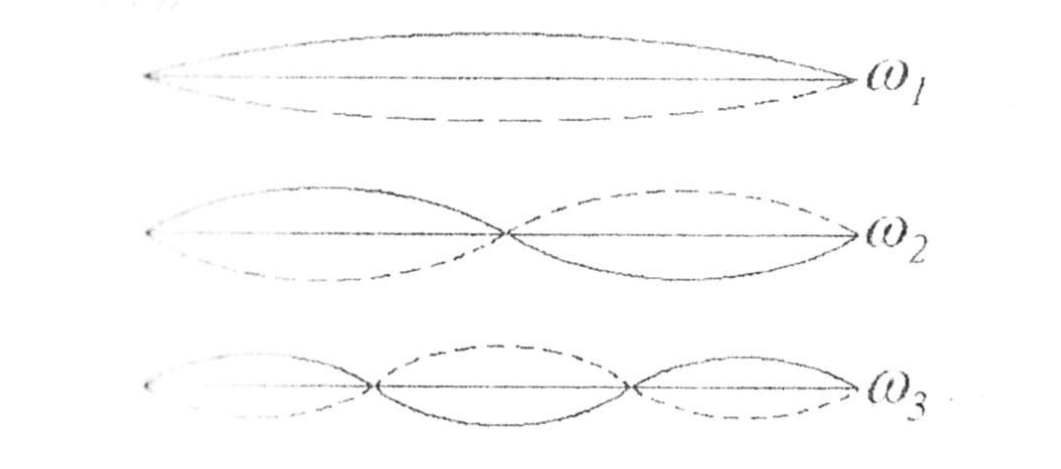
\includegraphics [width = 13cm] {Lab_6_2.png}
        \caption{\centering Схема форм искривлений вала.}
        \label{im2}
    \end{figure}
    
    \newpage
    
    \section{Результаты экспериментов}
    
    Далее представлены значения величин полученных в ходе эксперимента. Все замеры производились три раза. Теоретические рассчеты и экспериментальные результаты представлены в таблице \ref{tb4}.
    
    \begin{longtable}{| M{2cm} | M{3cm} | M{1.5cm} | M{1.5cm} | M{1.5cm} | M{1.5cm} | M{2.5cm} |}
        \caption{\centering Экспериментальные значения критических угловых скоростей.}
        \label{tb4} \\
        \hline
        \multirow{2}{*}{Величина} &
        \multirow{2}{*}{Теория} &
        \multicolumn{4}{M{7.3cm}|}{Эксперимент} &
        \multirow{2}{*}{Размерность} \\
        \cline{3-6}
        & & №1 & №2 & №3 & Среднее & \\
        \hline
        $\omega_{1}$ & $50,19 \pm 2,84$ & 52,77 & 56,55 & 54,66 & 54,66 & $1 / \text{с}$ \\
        $\omega_{2}$ & $200,77 \pm 11,37$ & 189,12 & 189,75 & 188,50 & 189,12 & $1 / \text{с}$ \\
        $\omega_{3}$ & $451,75 \pm 25,59$ & -- & -- & -- & -- & $1 / \text{с}$ \\
        \hline
    \end{longtable}
    
    Данные таблицы \ref{tb4} позволяют заключить, что теоретический рассчет оказался достаточно точным и относительно хорошо приблизил действительные характеристики установки. Также важно отметить, что неточности в рассчетах могут быть связаны с некорректным указанием модуля упругости материала вала (оригинальный вал был заменен на другой, со схожим модулем упругости).
    
    В результате проделанной работы были получены критические угловые частоты вращения вала, соответствующие различным формам его искривления. Все теоретические и практические результаты представлены выше.
    
    \newpage
    
\end{document}